\documentclass[PICOAPC.tex]{subfiles}

\begin{document}

%Enumerate the various signals in polarization. Use the frequency band + signals figure. The challenge is to dig out the faintest of all signals, the one due to $r$. This sets the tone for the entire 'signal decomposition' or 'component separation'.  Removing the galactic signal to unmask $r \lesssim 0.001$ is a challenge for all future experiments searching for $r$ at that level, and is a strong advantage of a space platform. The physics of galactic signals suggests complexities in their combined emission properties; the level of this complexity is not known. } 

\subsubsection{The Signal Separation Challenge}
\label{sec:separation_challenge}

Galactic emission dominates the sky's polarized intensity on large angular scales ($\ell \lesssim 10$), it dominates the cosmological $B$-modes signals for $\ell \lesssim 150$ for all allowed levels of $r$, and it is expected to be significant even at $\ell \simeq 1000$, posing challenge for reconstructing the $B$-mode signal from lensing. This is illustrated in Figs.~\ref{fig:clbb} and~\ref{fig:pico-channels-and-fg}, which show Galactic emission power spectra calculated for the cleanest -- that is, the least Galactic-emission-contaminated -- 60\% of the sky. But even in small patches of the sky, far from the Galactic plane and with the least foreground contamination, Galactic emission levels are substantial relative to an inflationary signal of $r \sim 0.01$~\cite{planckEB}. Separating the cosmological and Galactic emission signals is one of two primary challenges facing any next-decade experiment attempting to reach these levels of constraints on $r$ (the second is control of systematic uncertainties).

\begin{figure}[ht]
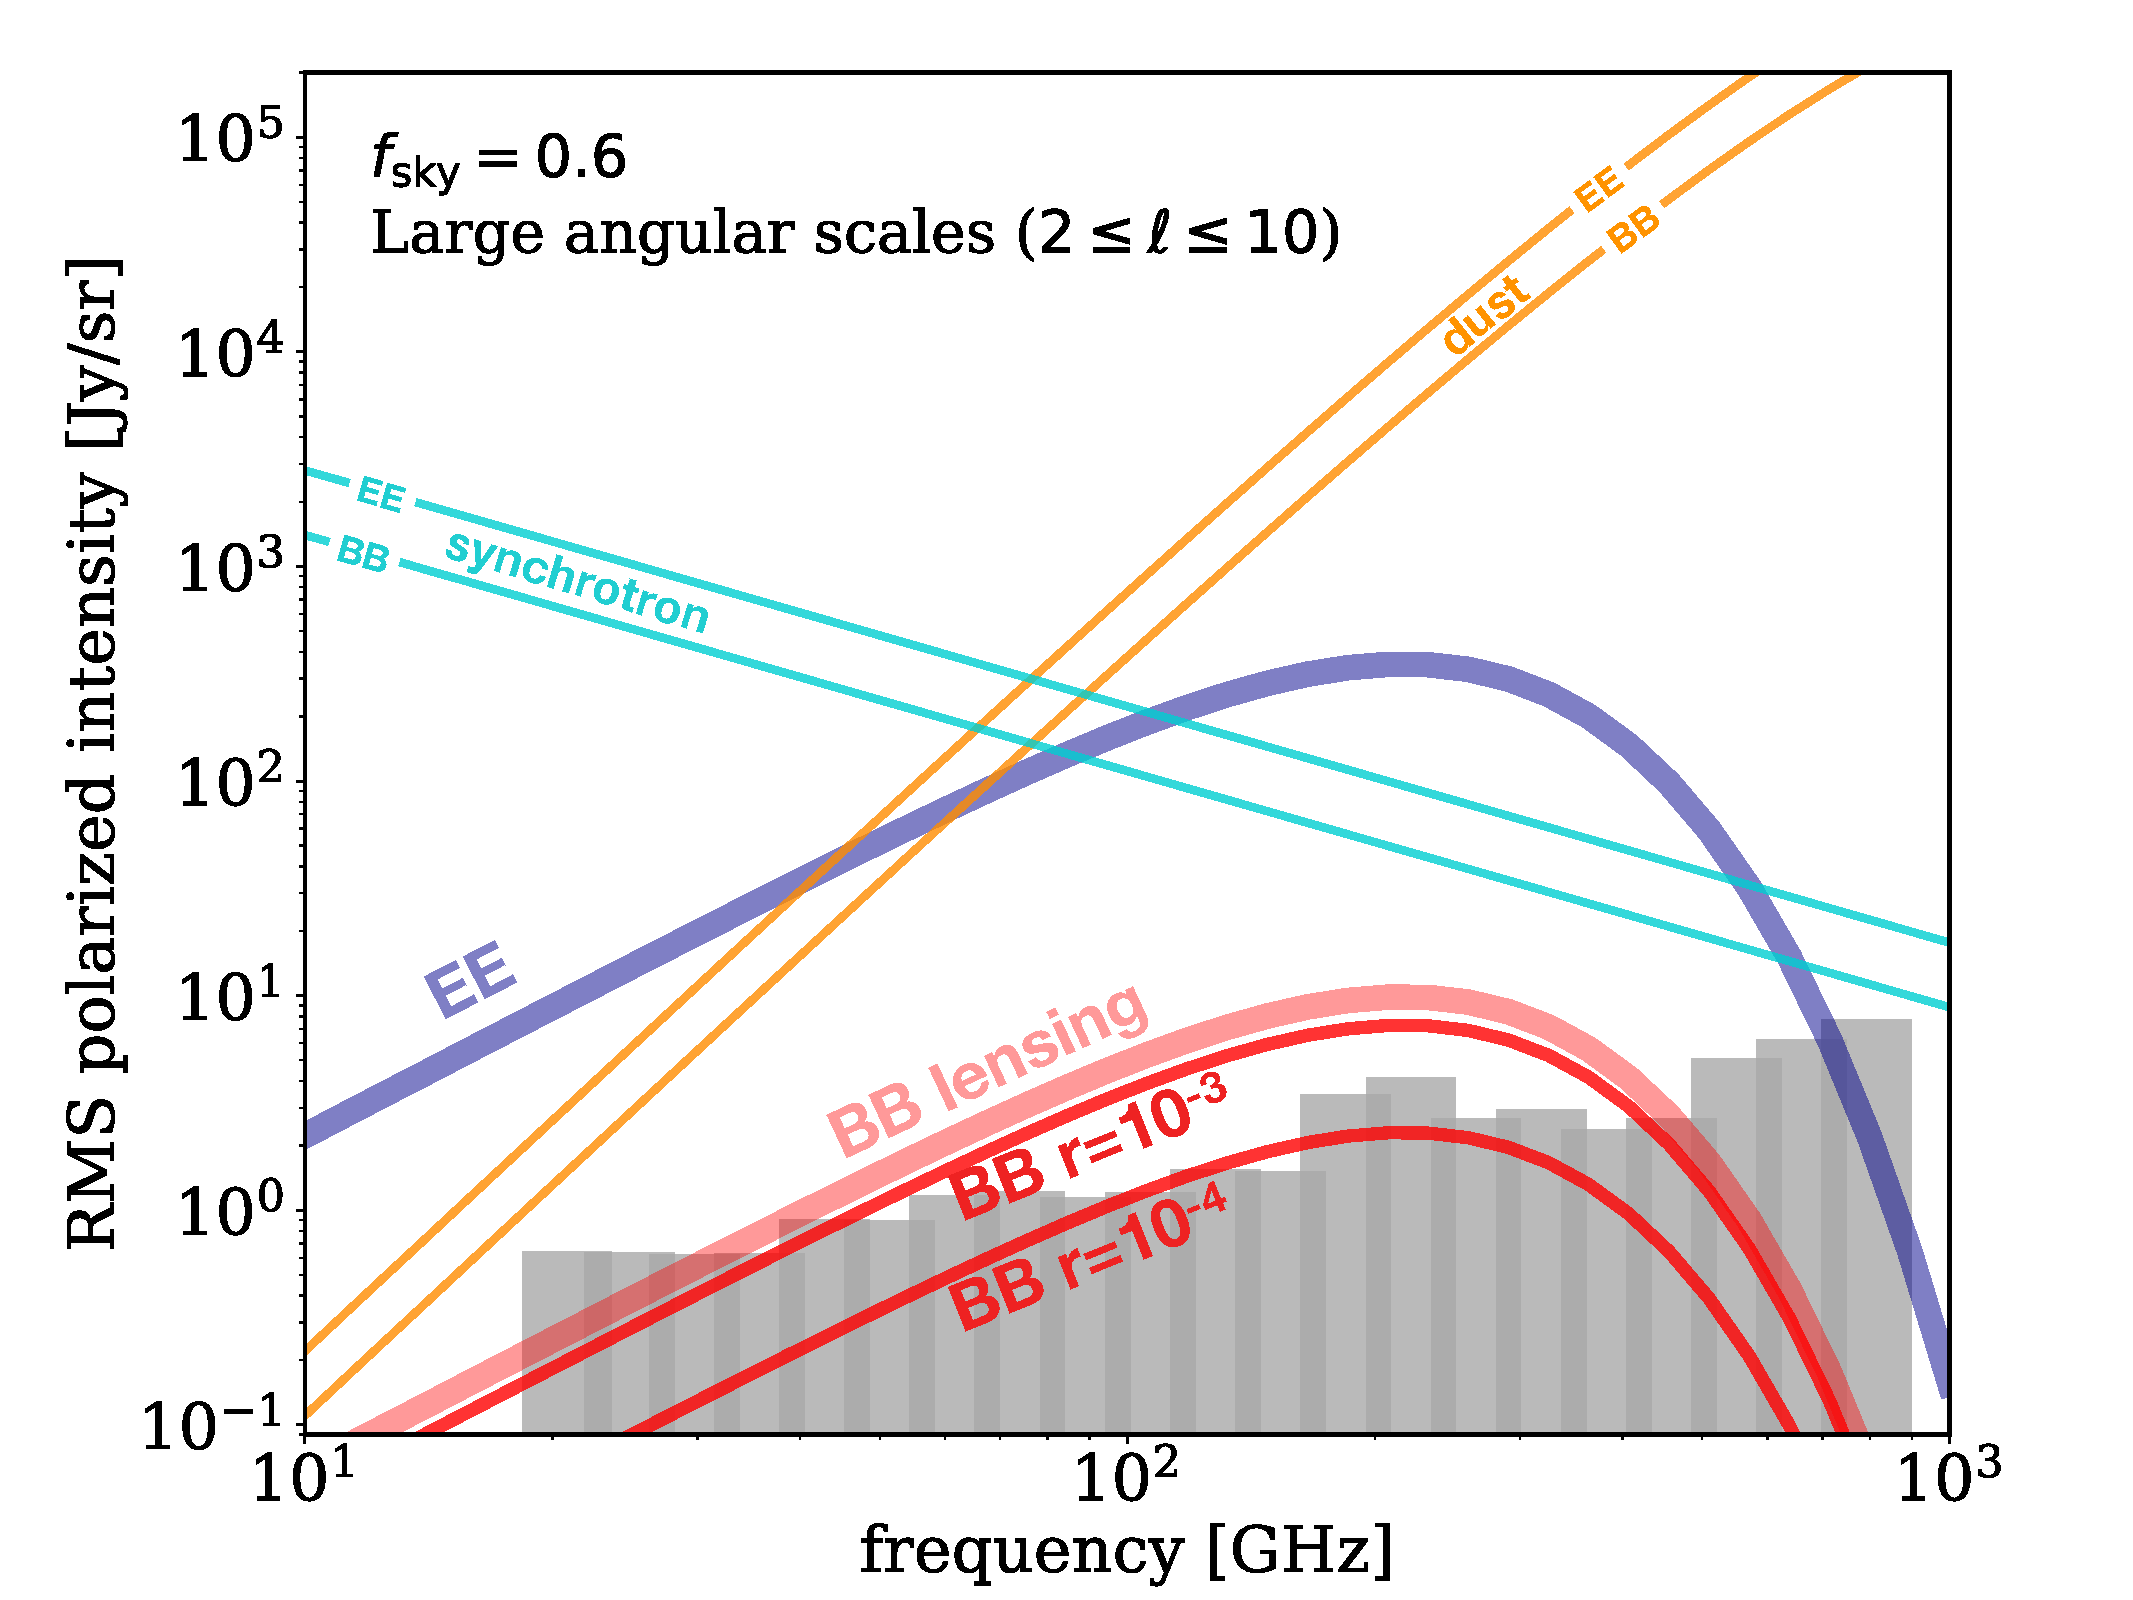
\includegraphics[width=0.49\textwidth]{images/sensitivity_vs_frequency_Jan3_2019_large_scale_v2.pdf}
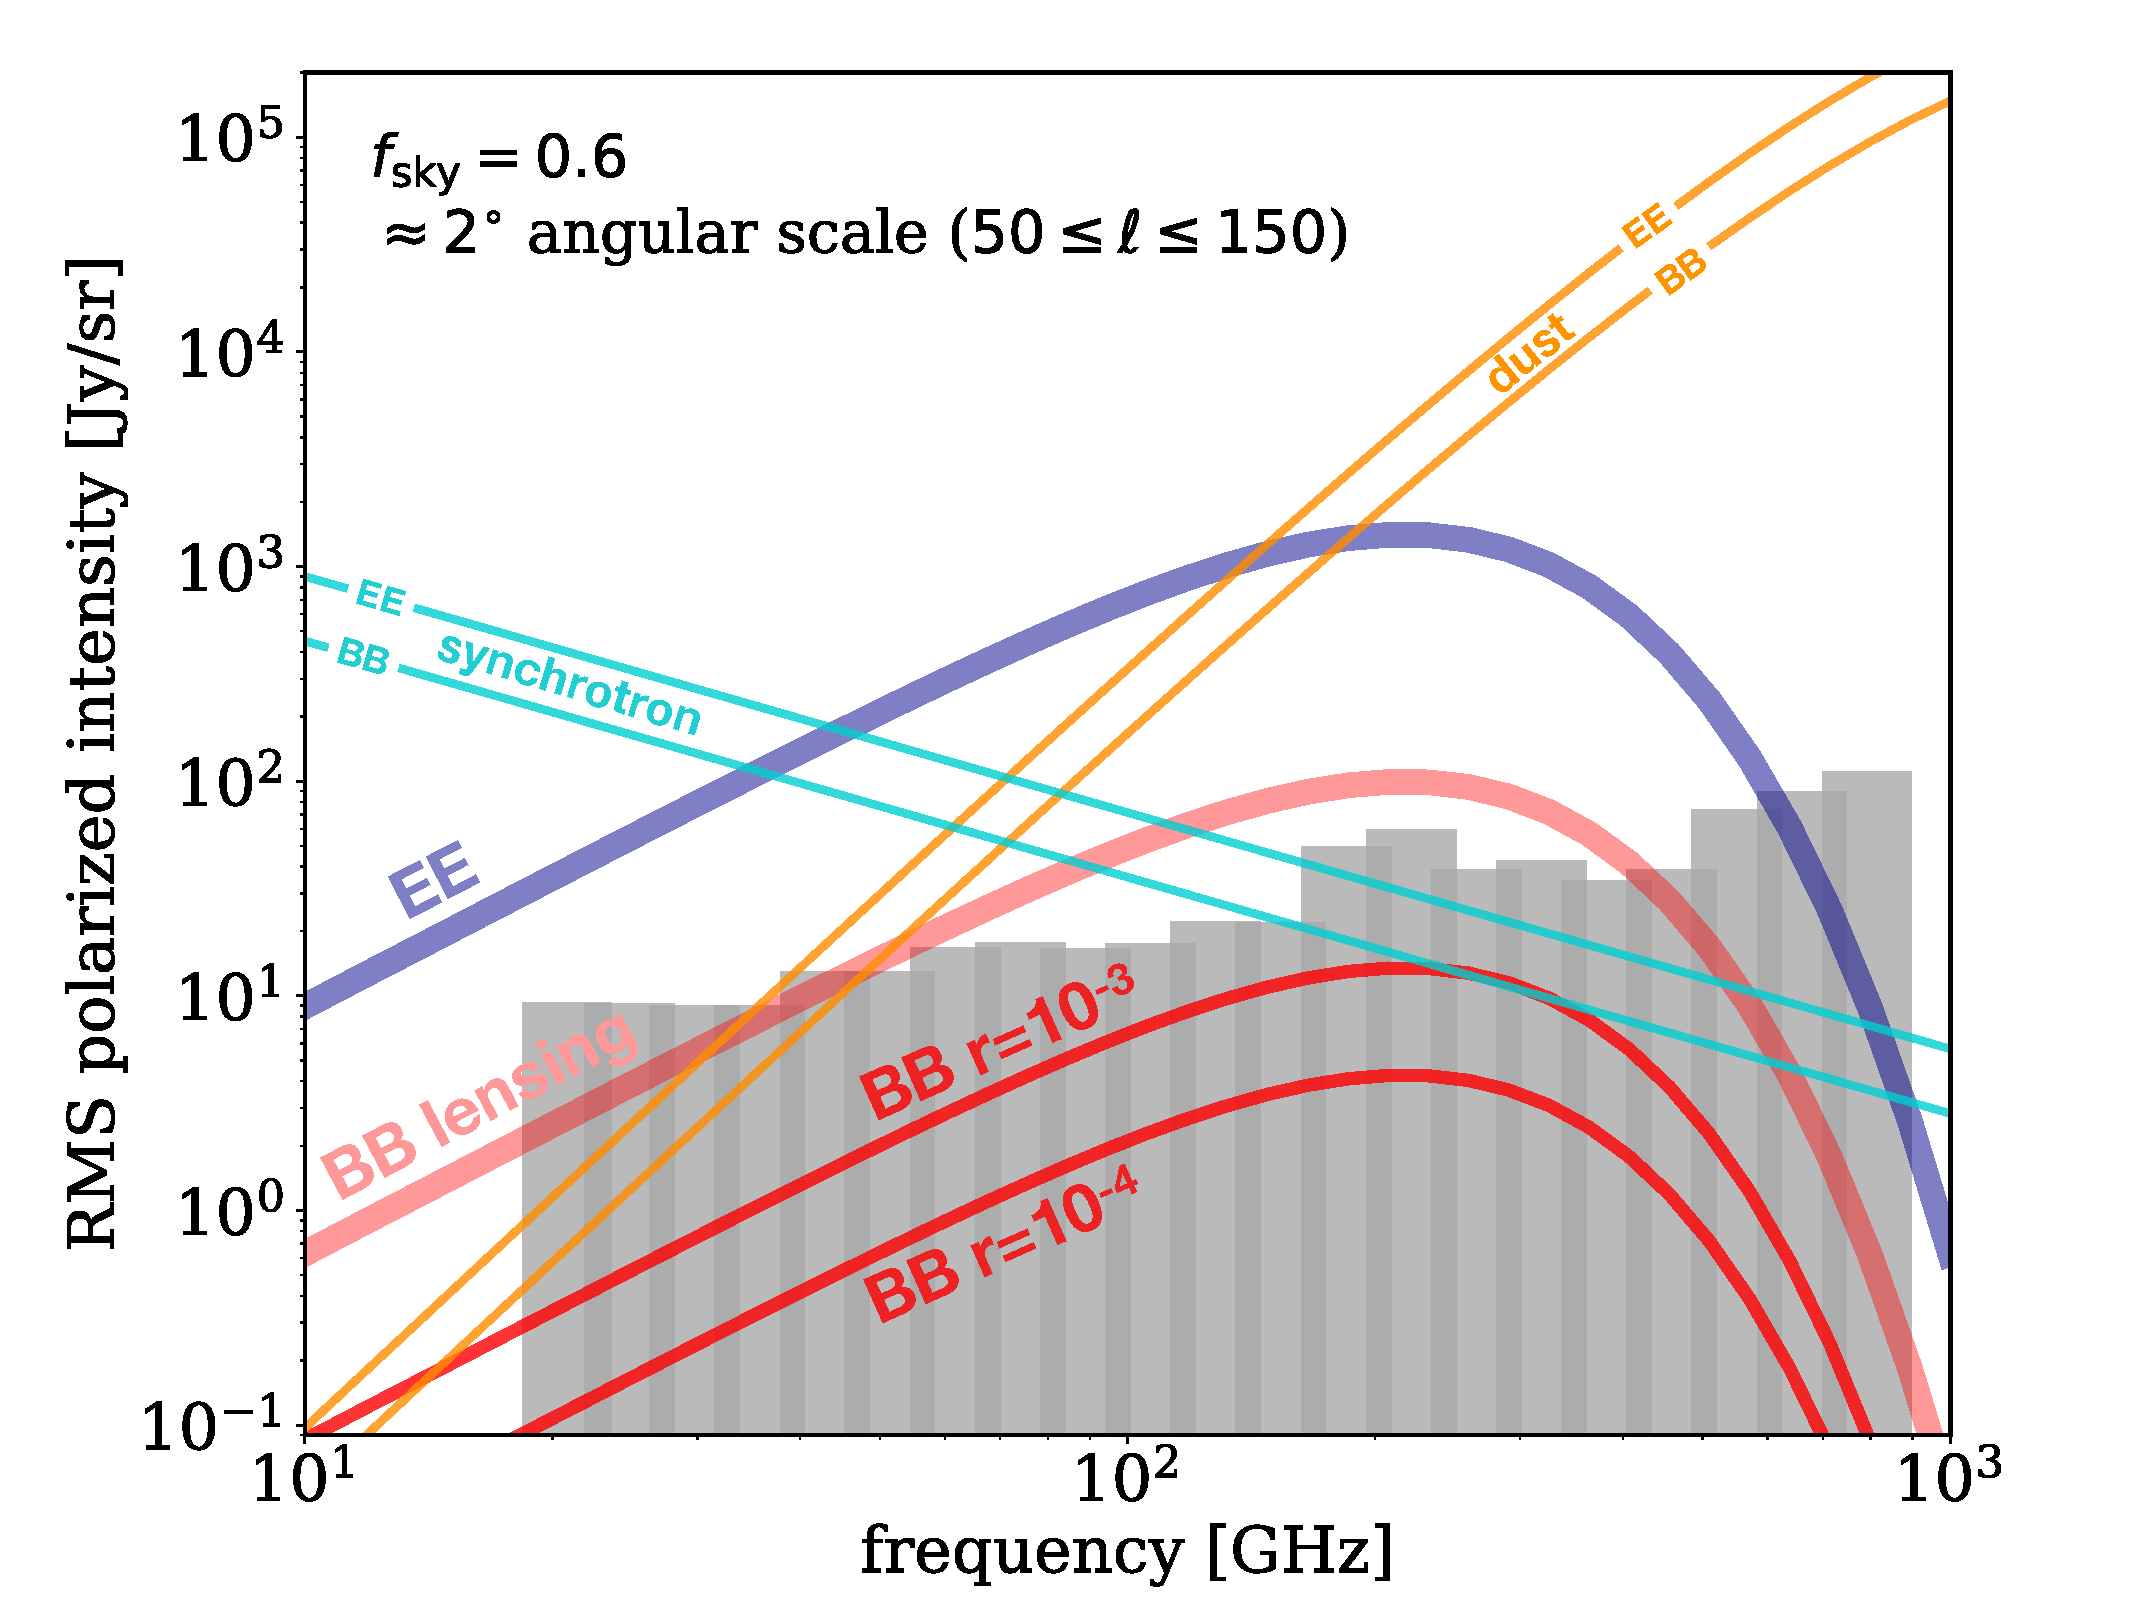
\includegraphics[width=0.49\textwidth]{images/sensitivity_vs_frequency_Jan3_2019_2deg_scale_v2.pdf}
\vspace{-0.1in}
\caption{\captiontext
Polarization $BB$ spectra of Galactic synchrotron and dust, compared to CMB polarization $EE$ and $BB$ spectra of different origins for two values of $r$ and for two ranges of angular scales: large-scale, $\ell \leq 10$, corresponding to the reionization peak (left panel); and intermediate scales $50 \leq \ell \leq 150$, corresponding to the recombination peak (right panel). 
Data from \planck\ indicate that for Galactic emission the level of the $E$-mode is approximately twice that of $B$~\cite{planckEB}.
The PICO baseline noise (grey bands) is low compared to the Galactic emission components, and thus they will be measured with high \ac{SNR} in many frequency bands.
\label{fig:pico-channels-and-fg} }
\vspace{-0.05in}
\end{figure}

To investigate the efficacy of PICO in addressing the foreground-separation challenge, we used both an analytic forecast and map-domain simulations; a complete description is given in~\citet{picoreport}. Here we present results only from the more conservative map-domain analysis. In this analysis we simulate sky maps that are constrained by available data, but otherwise have a mixture of foreground properties; we `observe' these maps just like a realistic experiment would do, and then apply foreground separation techniques to separate the Galactic and CMB emissions.  
Our results indicate that: \\
$\bullet$ the combination of PICO's sensitivity and broad frequency coverage are effective in foreground removal and that PICO will reach the requirement of $r = 5\times 10^{-4} \,(5\sigma)$; see Figure~\ref{fig:nilc};
$\bullet$ the high frequency bands, above 400~GHz, may be essential for proper subtraction of foregrounds; see Figure~\ref{fig:commander}. \\
Among all next decade experiments, PICO is best suited to handle and model the foregrounds because it has more frequency bands than any other experiment, because it has the lowest noise, and because it has full sky coverage, giving access to several independent small regions that are very low in dust emission. This is a distinct advantage relative to CMB-S4, which targets a single patch of the sky, and relative to liteBIRD, which does not have frequency bands above 400~GHz. 

\begin{figure}[h]
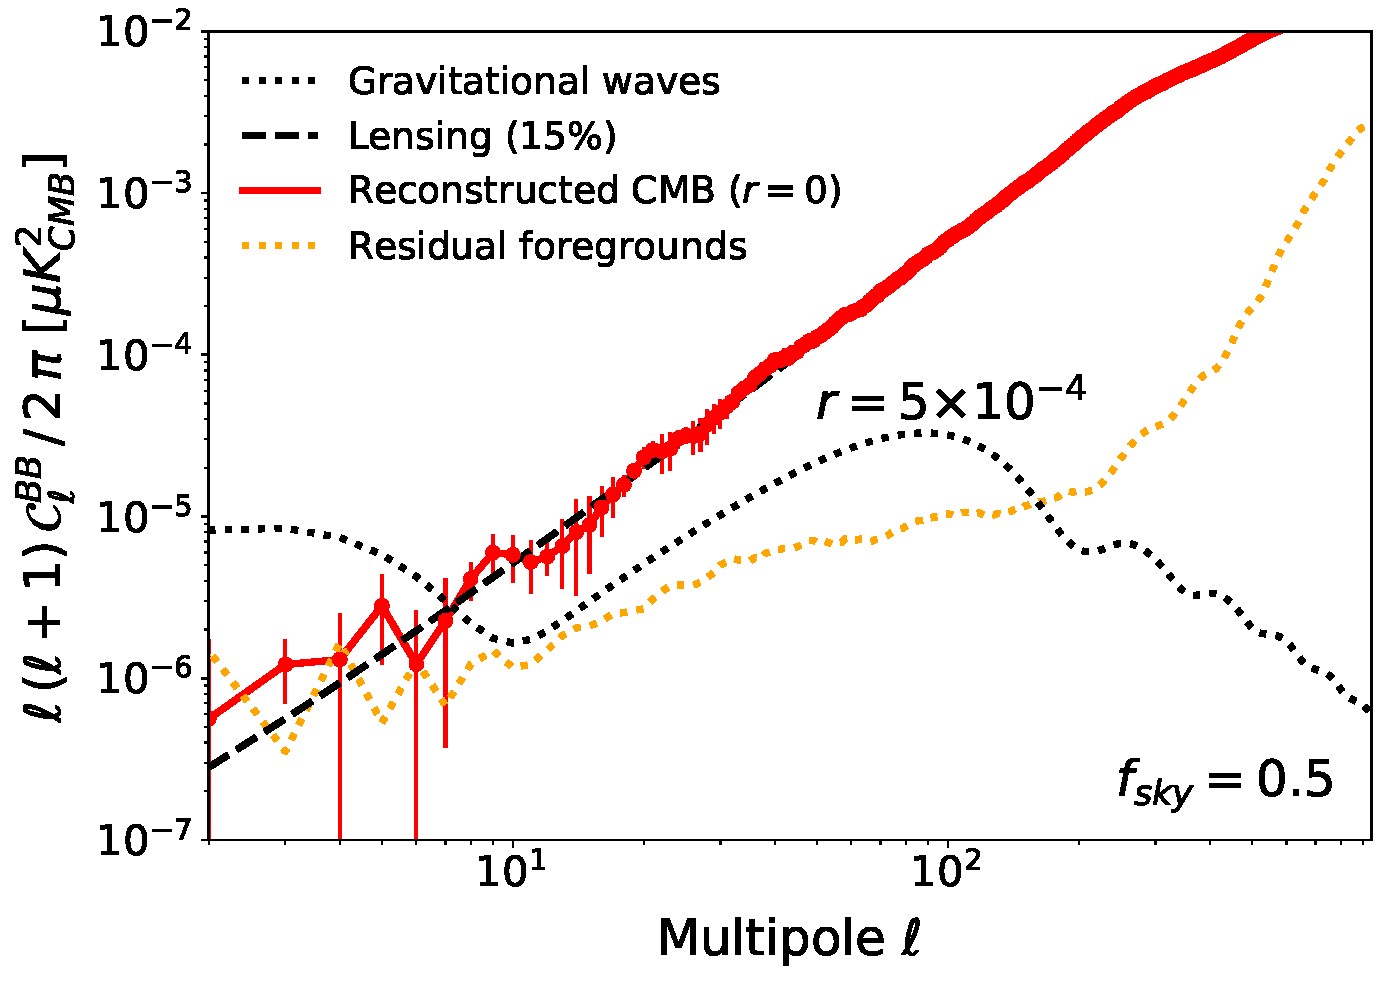
\includegraphics[width=3.2in]{images/gnilc_9092_residual.pdf}
\hspace{0.1in}
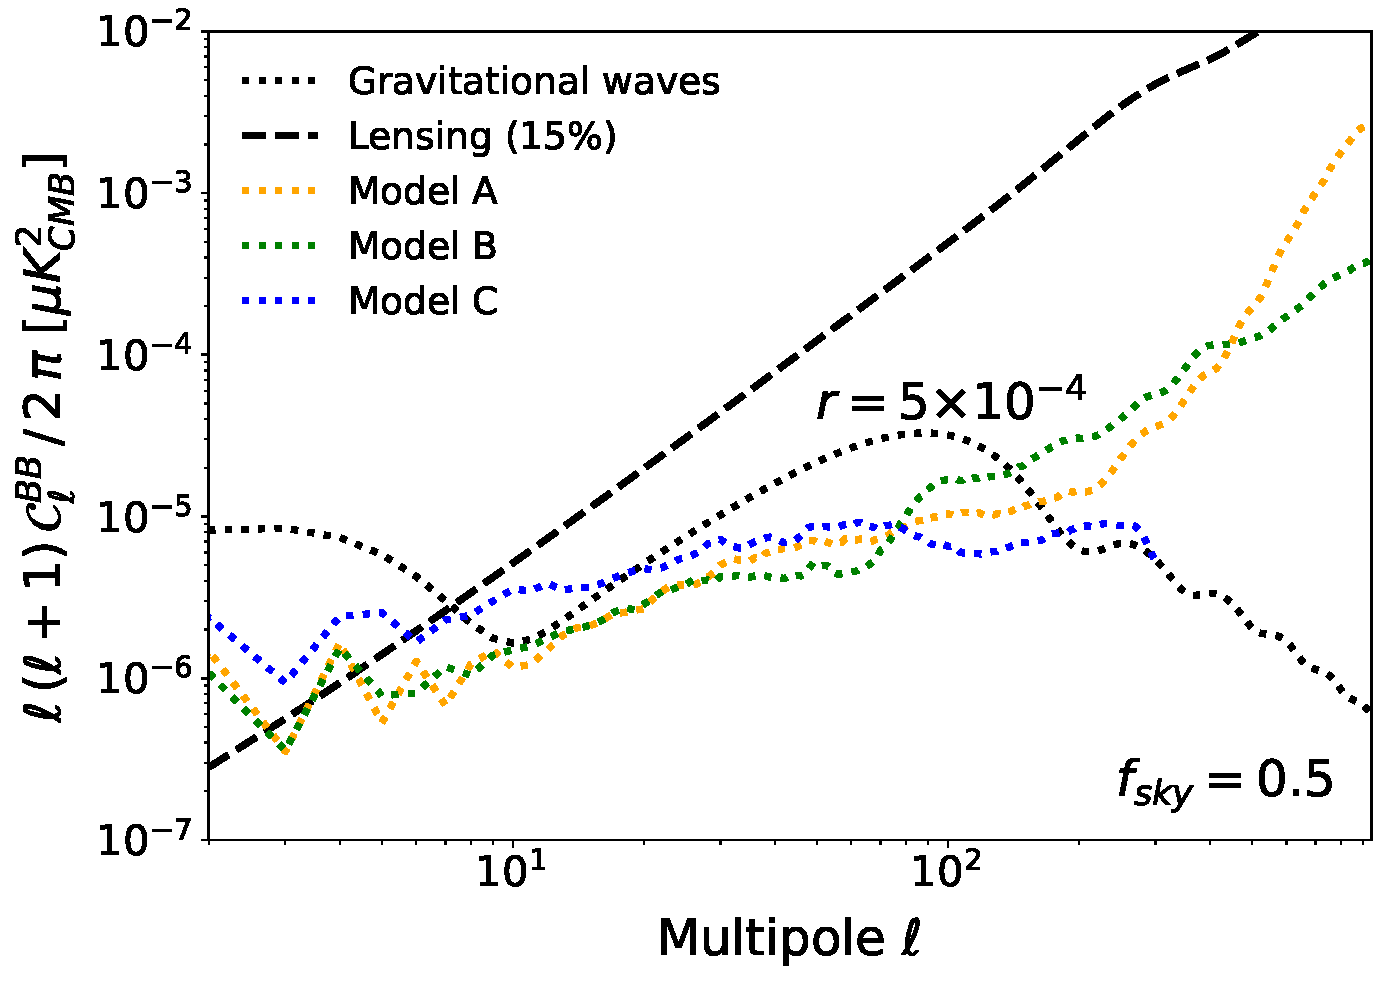
\includegraphics[width=3.2in]{images/gnilc_several_residuals.pdf}
\vspace{-0.3in}
\caption{\captiontext Angular power spectra of $BB$ due to the CMB and of residual foregrounds after an end-to-end map-based foreground-separation exercise. The PICO low noise levels and breadth in frequency coverage enable separation of model A foregrounds such that the residual foreground spectrum (left, yellow dotted) is a factor of ten (four) below a $BB$ inflationary signal with $r=5\times10^{-4}$ (black dotted) at $\ell=5 (80)$. Within errors, the recovered CMB (red) matches the input CMB, which consists of only lensing $BB$ (dashed black), over all angular scales $\ell \gtrsim 6$.  The results for model B are similar (right, green dots), while model C has somewhat higher residuals at low $\ell$. In this exercise we used 50\% of the sky. Lower foreground residual levels are obtainable with smaller, cleaner patches of $\sim$5\% of sky, which would reduce the residual foregrounds at $\ell \simeq 80$. 
\label{fig:nilc} } 
\vspace{-0.05in}
\end{figure}

\begin{figure}
%\hspace{-0.1in}
%\parbox{4.5in}
\centering
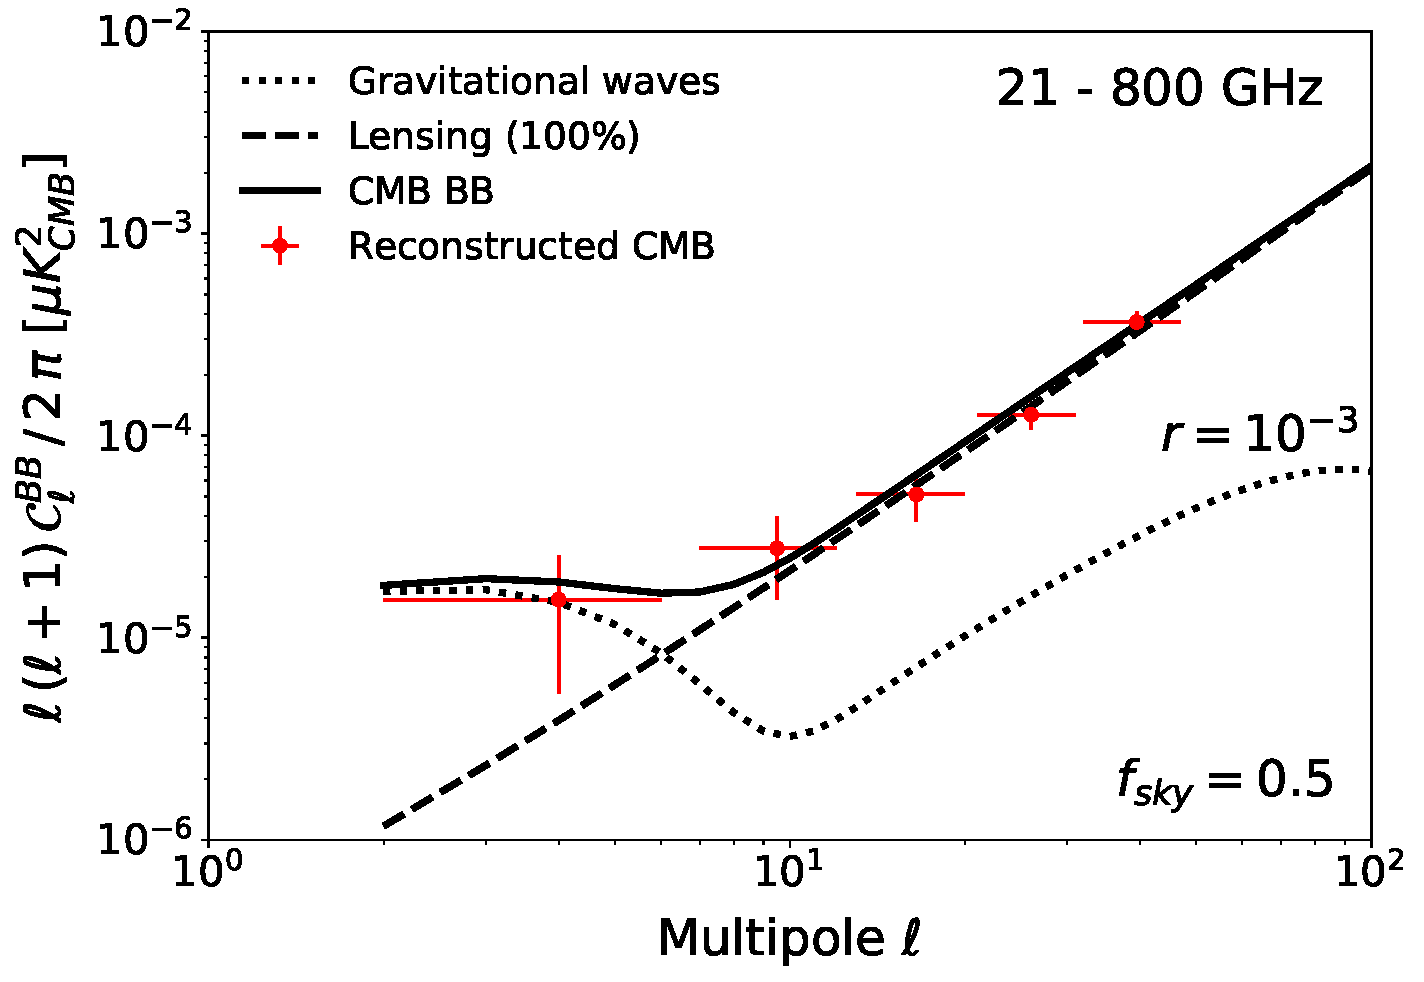
\includegraphics[width=3in]{images/commander_pico_baseline.pdf}
\hspace{-0.0in}
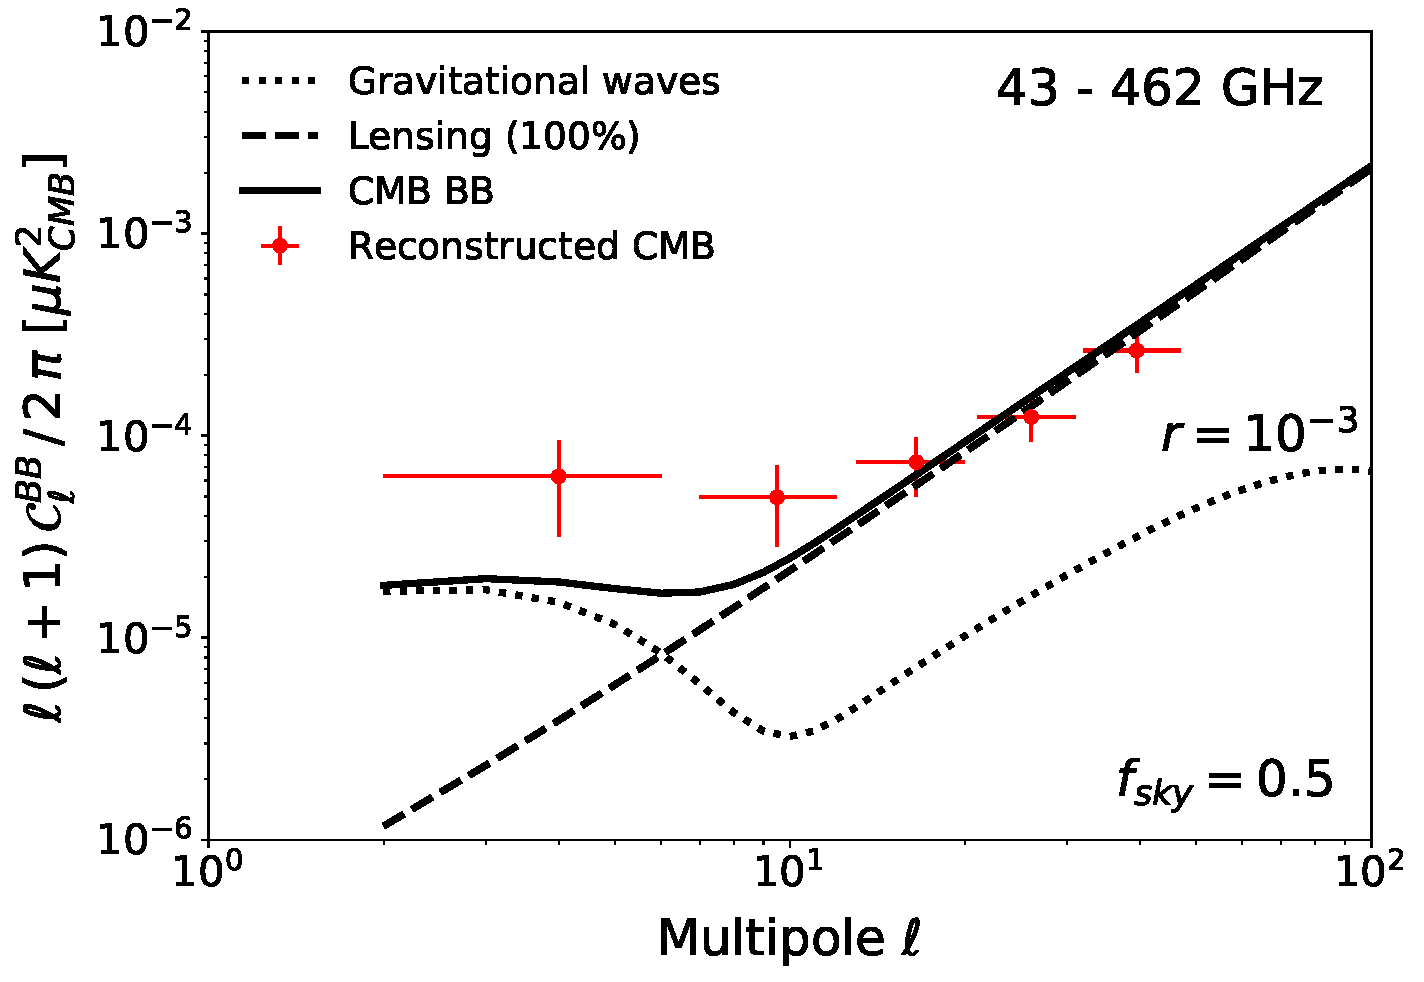
\includegraphics[width=3in]{images/commander_pico_descoped.pdf}
%\hspace{0.in}
%\parbox{2.0in}{
\vspace{-0.1in}
\caption{\captiontext
{\bf Left:} Foreground separation with all of PICO's 21 frequency bands recovers the input CMB $BB$ power spectrum (solid black) without bias (red). The input CMB spectrum has a contribution from lensing (dashed) and an inflationary signal with $r=0.001$ (dotted). This exercise uses a parametric approach~\citep{eriksen/etal:2008} with foregrounds varying on 4$^\circ$ pixels, and using 50\% sky fraction. {\bf Right:} Running the same foreground separation algorithm on the same sky but using only PICO's bands between 43 and 462~GHz produces an output spectrum (red) that is biased at low multipoles relative to the input. With real data, such a bias would be erroneously interpreted as a higher value of $r$. 
\label{fig:commander}}
\vspace{-0.1in}
\end{figure}


\end{document}

%\begin{figure}[!htb]
%\centering
%\includegraphics[width=4cm]{images/example}
%\caption{example}
%\label{fig:im_3}
%\end{figure}

%The most important lesson arising from our exercise is that more work is required to ascertain that levels of $r \lesssim 0.001$ can be determined robustly on the largest angular scales, that is from the reionization peak.  Fig.~\ref{fig:nilc} shows results from the NILC analysis. For several of the sky models the power spectra of the residual level of foregrounds -- that is the level of foregrounds remaining in the map after foreground separation -- is below the cosmological \ac{IGW} level with $r =0.003$. For a minority of the models, the residual is higher at $\ell \lesssim 20$. Results from GNILC, shown in Fig.~\ref{fig:gnilc}, are similar. In all cases, the analyses are carried out using 60\% of the sky, the results shown are from one realization, and that no further optimization of the basic foreground separation technique has yet been applied. 

%More work is also required to understand the necessary span of frequencies required. Fig.~\ref{fig:psm_mr} shows that removing several of PICO's frequency bands, in this case the three highest, significantly biases the extracted $BB$ power spectrum, particularly at the lowest $\ell$ values. This result should not be interpreted as conclusively demonstrating that a frequency span up to 800 GHz has been proven to be essential. At this point of time, different input sky models, coupled to different foreground separation techniques may yield different results. Rather, the conclusion is that further improvement in our modeling and analysis is required. 



%The baseline design of PICO has 21 channels observing the sky in the 20\,GHz to 800\,GHz frequency range (Fig.~\ref{fig:pico-channels-and-fg}). By analysing how the total emission varies across frequency bands, one can infer the detailed emission properties of the various emission components, form linear combinations of the observations that maximise the contribution of a component of interest while minimising contamination by the others and by instrumental noise, and understand the properties of the foregrounds to evaluate potential residuals in the CMB B-mode map. Various such techniques have been successfully used in previous CMB observations such as those of the Planck mission. Building on this existing expertise, we have carried out map based simulations within a ``data challenge'' framework to assess the capacity of PICO to measure the main signal of interest (CMB primordial B-modes). In this process one group prepares sets of simulated maps for different models of foreground emission of varying complexity from optimistic to pessimistic, which are placed in a shared area. These are then re-analyzed by multiple individuals and groups employing various different component separation algorithms.

